% Options for packages loaded elsewhere
\PassOptionsToPackage{unicode}{hyperref}
\PassOptionsToPackage{hyphens}{url}
\PassOptionsToPackage{dvipsnames,svgnames,x11names}{xcolor}
%
\documentclass[
  12pt,
  a4paper,
  oneside]{tesesusp}

\usepackage{amsmath,amssymb}
\usepackage{iftex}
\ifPDFTeX
  \usepackage[T1]{fontenc}
  \usepackage[utf8]{inputenc}
  \usepackage{textcomp} % provide euro and other symbols
\else % if luatex or xetex
  \usepackage{unicode-math}
  \defaultfontfeatures{Scale=MatchLowercase}
  \defaultfontfeatures[\rmfamily]{Ligatures=TeX,Scale=1}
\fi
\usepackage{lmodern}
\ifPDFTeX\else  
    % xetex/luatex font selection
  \setmainfont[]{Arial}
  \setsansfont[]{Arial}
\fi
% Use upquote if available, for straight quotes in verbatim environments
\IfFileExists{upquote.sty}{\usepackage{upquote}}{}
\IfFileExists{microtype.sty}{% use microtype if available
  \usepackage[]{microtype}
  \UseMicrotypeSet[protrusion]{basicmath} % disable protrusion for tt fonts
}{}
\makeatletter
\@ifundefined{KOMAClassName}{% if non-KOMA class
  \IfFileExists{parskip.sty}{%
    \usepackage{parskip}
  }{% else
    \setlength{\parindent}{0pt}
    \setlength{\parskip}{6pt plus 2pt minus 1pt}}
}{% if KOMA class
  \KOMAoptions{parskip=half}}
\makeatother
\usepackage{xcolor}
\setlength{\emergencystretch}{3em} % prevent overfull lines
\setcounter{secnumdepth}{5}
% Make \paragraph and \subparagraph free-standing
\ifx\paragraph\undefined\else
  \let\oldparagraph\paragraph
  \renewcommand{\paragraph}[1]{\oldparagraph{#1}\mbox{}}
\fi
\ifx\subparagraph\undefined\else
  \let\oldsubparagraph\subparagraph
  \renewcommand{\subparagraph}[1]{\oldsubparagraph{#1}\mbox{}}
\fi

\usepackage{color}
\usepackage{fancyvrb}
\newcommand{\VerbBar}{|}
\newcommand{\VERB}{\Verb[commandchars=\\\{\}]}
\DefineVerbatimEnvironment{Highlighting}{Verbatim}{commandchars=\\\{\}}
% Add ',fontsize=\small' for more characters per line
\usepackage{framed}
\definecolor{shadecolor}{RGB}{241,243,245}
\newenvironment{Shaded}{\begin{snugshade}}{\end{snugshade}}
\newcommand{\AlertTok}[1]{\textcolor[rgb]{0.68,0.00,0.00}{#1}}
\newcommand{\AnnotationTok}[1]{\textcolor[rgb]{0.37,0.37,0.37}{#1}}
\newcommand{\AttributeTok}[1]{\textcolor[rgb]{0.40,0.45,0.13}{#1}}
\newcommand{\BaseNTok}[1]{\textcolor[rgb]{0.68,0.00,0.00}{#1}}
\newcommand{\BuiltInTok}[1]{\textcolor[rgb]{0.00,0.23,0.31}{#1}}
\newcommand{\CharTok}[1]{\textcolor[rgb]{0.13,0.47,0.30}{#1}}
\newcommand{\CommentTok}[1]{\textcolor[rgb]{0.37,0.37,0.37}{#1}}
\newcommand{\CommentVarTok}[1]{\textcolor[rgb]{0.37,0.37,0.37}{\textit{#1}}}
\newcommand{\ConstantTok}[1]{\textcolor[rgb]{0.56,0.35,0.01}{#1}}
\newcommand{\ControlFlowTok}[1]{\textcolor[rgb]{0.00,0.23,0.31}{#1}}
\newcommand{\DataTypeTok}[1]{\textcolor[rgb]{0.68,0.00,0.00}{#1}}
\newcommand{\DecValTok}[1]{\textcolor[rgb]{0.68,0.00,0.00}{#1}}
\newcommand{\DocumentationTok}[1]{\textcolor[rgb]{0.37,0.37,0.37}{\textit{#1}}}
\newcommand{\ErrorTok}[1]{\textcolor[rgb]{0.68,0.00,0.00}{#1}}
\newcommand{\ExtensionTok}[1]{\textcolor[rgb]{0.00,0.23,0.31}{#1}}
\newcommand{\FloatTok}[1]{\textcolor[rgb]{0.68,0.00,0.00}{#1}}
\newcommand{\FunctionTok}[1]{\textcolor[rgb]{0.28,0.35,0.67}{#1}}
\newcommand{\ImportTok}[1]{\textcolor[rgb]{0.00,0.46,0.62}{#1}}
\newcommand{\InformationTok}[1]{\textcolor[rgb]{0.37,0.37,0.37}{#1}}
\newcommand{\KeywordTok}[1]{\textcolor[rgb]{0.00,0.23,0.31}{#1}}
\newcommand{\NormalTok}[1]{\textcolor[rgb]{0.00,0.23,0.31}{#1}}
\newcommand{\OperatorTok}[1]{\textcolor[rgb]{0.37,0.37,0.37}{#1}}
\newcommand{\OtherTok}[1]{\textcolor[rgb]{0.00,0.23,0.31}{#1}}
\newcommand{\PreprocessorTok}[1]{\textcolor[rgb]{0.68,0.00,0.00}{#1}}
\newcommand{\RegionMarkerTok}[1]{\textcolor[rgb]{0.00,0.23,0.31}{#1}}
\newcommand{\SpecialCharTok}[1]{\textcolor[rgb]{0.37,0.37,0.37}{#1}}
\newcommand{\SpecialStringTok}[1]{\textcolor[rgb]{0.13,0.47,0.30}{#1}}
\newcommand{\StringTok}[1]{\textcolor[rgb]{0.13,0.47,0.30}{#1}}
\newcommand{\VariableTok}[1]{\textcolor[rgb]{0.07,0.07,0.07}{#1}}
\newcommand{\VerbatimStringTok}[1]{\textcolor[rgb]{0.13,0.47,0.30}{#1}}
\newcommand{\WarningTok}[1]{\textcolor[rgb]{0.37,0.37,0.37}{\textit{#1}}}

\providecommand{\tightlist}{%
  \setlength{\itemsep}{0pt}\setlength{\parskip}{0pt}}\usepackage{longtable,booktabs,array}
\usepackage{calc} % for calculating minipage widths
% Correct order of tables after \paragraph or \subparagraph
\usepackage{etoolbox}
\makeatletter
\patchcmd\longtable{\par}{\if@noskipsec\mbox{}\fi\par}{}{}
\makeatother
% Allow footnotes in longtable head/foot
\IfFileExists{footnotehyper.sty}{\usepackage{footnotehyper}}{\usepackage{footnote}}
\makesavenoteenv{longtable}
\usepackage{graphicx}
\makeatletter
\def\maxwidth{\ifdim\Gin@nat@width>\linewidth\linewidth\else\Gin@nat@width\fi}
\def\maxheight{\ifdim\Gin@nat@height>\textheight\textheight\else\Gin@nat@height\fi}
\makeatother
% Scale images if necessary, so that they will not overflow the page
% margins by default, and it is still possible to overwrite the defaults
% using explicit options in \includegraphics[width, height, ...]{}
\setkeys{Gin}{width=\maxwidth,height=\maxheight,keepaspectratio}
% Set default figure placement to htbp
\makeatletter
\def\fps@figure{htbp}
\makeatother
\newlength{\cslhangindent}
\setlength{\cslhangindent}{1.5em}
\newlength{\csllabelwidth}
\setlength{\csllabelwidth}{3em}
\newlength{\cslentryspacingunit} % times entry-spacing
\setlength{\cslentryspacingunit}{\parskip}
\newenvironment{CSLReferences}[2] % #1 hanging-ident, #2 entry spacing
 {% don't indent paragraphs
  \setlength{\parindent}{0pt}
  % turn on hanging indent if param 1 is 1
  \ifodd #1
  \let\oldpar\par
  \def\par{\hangindent=\cslhangindent\oldpar}
  \fi
  % set entry spacing
  \setlength{\parskip}{#2\cslentryspacingunit}
 }%
 {}
\usepackage{calc}
\newcommand{\CSLBlock}[1]{#1\hfill\break}
\newcommand{\CSLLeftMargin}[1]{\parbox[t]{\csllabelwidth}{#1}}
\newcommand{\CSLRightInline}[1]{\parbox[t]{\linewidth - \csllabelwidth}{#1}\break}
\newcommand{\CSLIndent}[1]{\hspace{\cslhangindent}#1}

% tesesusp.cls, v-0.0.1

% Based on 'bntex2ppgsi.cls' and 'abntex2.csl'.
% See <https://www.overleaf.com/project/64f7bdf1641ad4a3a8482800>.
% to learn more.

% Language (options: "brazil", "english")
% \usepackage[english]{babel}

% Document settings

% \documentclass[
% 	12pt,
% 	% openright, % Chapters begin on odd pages.
% 	oneside,
% 	a4paper,
% 	%% Options of the ABNTeX2 class
% 	%% 'TITLE' = titles converted to uppercase letters.
% 	chapter=TITLE,
% 	section=TITLE,
% 	subsection=TITLE,
% 	subsubsection=TITLE,
% 	%% Options of the Babel Package
% 	brazil, % Additional Language for Hyphenation.
% 	% spanish, % Additional Language for Hyphenation.
% 	english % The last language is the main one in the document.
% 	]{tesesusp}

% Load packages

\usepackage{abstract}
\usepackage{algorithm}
\usepackage[noend]{algpseudocode}
\usepackage{babel}
\usepackage{color}
\usepackage{graphicx}
\usepackage{indentfirst}
\usepackage[utf8]{inputenc}
\usepackage{lastpage}
\usepackage{mdwlist}
\usepackage{microtype}
\usepackage{pdfpages}
\usepackage[dvipsnames]{xcolor}

% See <https://getbootstrap.com/docs/4.0/utilities/colors/>.
\definecolor{quarto-blue}{HTML}{2780E3}
\definecolor{quarto-lighter-blue}{HTML}{ECF4FC}
\definecolor{quarto-orange}{HTML}{FF7518}
\definecolor{quarto-ligther-orange}{HTML}{FFF3EB}
\definecolor{quarto-red}{HTML}{D9534F}
\definecolor{quarto-ligther-red}{HTML}{FCF1F1}
\definecolor{quarto-green}{HTML}{3FB618}
\definecolor{quarto-ligther-green}{HTML}{EFF9EB}
\definecolor{quarto-purple}{HTML}{7D12BA}
\definecolor{quarto-gray}{HTML}{A3A3A3}
\definecolor{quarto-medium-gray}{HTML}{CFD0D1}
\definecolor{quarto-ligther-gray}{HTML}{F1F3F5}

\definecolor{bs-link-color}{HTML}{39729E}
% tesesusp.cls, v-0.0.1

% Based on 'bntex2ppgsi.cls', 'abntex2.csl' and on USP guidelines to create
% thesis and dissertation documents.
% See <https://www.overleaf.com/project/64f7bdf1641ad4a3a8482800>
% and <https://teses.usp.br/index.php?option=com_content&
%      view=article&id=52&Itemid=67&lang=en>
% to learn more.

% ----------------------------------------------------------------------
% Cover
% ----------------------------------------------------------------------

\instituicao{
	UNIVERSITY OF SÃO PAULO
	\par
	[DEPARTAMENT/SCHOOL]
	\par
	[GRADUATE PROGRAM]
}

\local{São Paulo}
\orientador{Prof. Dr. [SUPERVISOR'S FULL NAME}
\coorientador{Prof. Dr. [CO-SUPERVISOR'S FULL NAME]}
\tipotrabalho{Type of thesis}

% ----------------------------------------------------------------------
% Title page
% ----------------------------------------------------------------------

%% Avoid using this page for qualification exams.
\preambulo{
  Original version

  \vspace{1cm}

  [DISSERTATION/THESIS] presented to the [SCHOOL/DEPARTMENT] at the University of São Paulo, as part of the requirements for the degree of [TYPE OF DEGREE] by the [GRADUATE PROGRAM].

  \vspace{0.5cm}

  Area of Concentration: [AREA OF CONCENTRATION].

  \vspace{1cm}

  Revised version incorporating the changes requested by the examining committee on [DATE]. The original version is held in the reserved collection at the [SCHOOL/DEPARTAMENT] Library and in the Digital Library of Theses and Dissertations of the University of São Paulo (BDTD-USP), in accordance with \href{https://leginf.usp.br/?resolucao=resolucao-copgr-no-6018-de-13-de-outubro-de-2011}{Resolution CoPGr 6018, dated October 13, 2011}.

  \vspace{1cm}

  Supervisor: Prof. Dr. [SUPERVISOR'S FULL NAME]

  \vspace{0.25cm}

  Co-Supervisor: Prof. Dr. [CO-SUPERVISOR'S FULL NAME]
}

% ----------------------------------------------------------------------
% Final PDF appearance settings (change only if necessary)
% ----------------------------------------------------------------------

\usepackage{array}
\usepackage{float}

\floatplacement{table}{H}
\newcolumntype{P}[1]{>{\centering\arraybackslash}p{#1}}

\setlength{\parindent}{1.25cm}
\setlength{\parskip}{0cm}
\renewcommand{\baselinestretch}{1.5}

% \makeindex

\clubpenalty10000
\widowpenalty10000
\displaywidowpenalty10000
\usepackage{booktabs}
\usepackage{longtable}
\usepackage{array}
\usepackage{multirow}
\usepackage{wrapfig}
\usepackage{float}
\usepackage{colortbl}
\usepackage{pdflscape}
\usepackage{tabu}
\usepackage{threeparttable}
\usepackage{threeparttablex}
\usepackage[normalem]{ulem}
\usepackage{makecell}
\usepackage{xcolor}
\makeatletter
\@ifpackageloaded{tcolorbox}{}{\usepackage[skins,breakable]{tcolorbox}}
\@ifpackageloaded{fontawesome5}{}{\usepackage{fontawesome5}}
\definecolor{quarto-callout-color}{HTML}{909090}
\definecolor{quarto-callout-note-color}{HTML}{0758E5}
\definecolor{quarto-callout-important-color}{HTML}{CC1914}
\definecolor{quarto-callout-warning-color}{HTML}{EB9113}
\definecolor{quarto-callout-tip-color}{HTML}{00A047}
\definecolor{quarto-callout-caution-color}{HTML}{FC5300}
\definecolor{quarto-callout-color-frame}{HTML}{acacac}
\definecolor{quarto-callout-note-color-frame}{HTML}{4582ec}
\definecolor{quarto-callout-important-color-frame}{HTML}{d9534f}
\definecolor{quarto-callout-warning-color-frame}{HTML}{f0ad4e}
\definecolor{quarto-callout-tip-color-frame}{HTML}{02b875}
\definecolor{quarto-callout-caution-color-frame}{HTML}{fd7e14}
\makeatother
\makeatletter
\makeatother
\makeatletter
\@ifpackageloaded{bookmark}{}{\usepackage{bookmark}}
\makeatother
\makeatletter
\@ifpackageloaded{caption}{}{\usepackage{caption}}
\AtBeginDocument{%
\ifdefined\contentsname
  \renewcommand*\contentsname{Table of contents}
\else
  \newcommand\contentsname{Table of contents}
\fi
\ifdefined\listfigurename
  \renewcommand*\listfigurename{List of Figures}
\else
  \newcommand\listfigurename{List of Figures}
\fi
\ifdefined\listtablename
  \renewcommand*\listtablename{List of Tables}
\else
  \newcommand\listtablename{List of Tables}
\fi
\ifdefined\figurename
  \renewcommand*\figurename{Figure}
\else
  \newcommand\figurename{Figure}
\fi
\ifdefined\tablename
  \renewcommand*\tablename{Table}
\else
  \newcommand\tablename{Table}
\fi
}
\@ifpackageloaded{float}{}{\usepackage{float}}
\floatstyle{ruled}
\@ifundefined{c@chapter}{\newfloat{codelisting}{h}{lop}}{\newfloat{codelisting}{h}{lop}[chapter]}
\floatname{codelisting}{Listing}
\newcommand*\listoflistings{\listof{codelisting}{List of Listings}}
\makeatother
\makeatletter
\@ifpackageloaded{caption}{}{\usepackage{caption}}
\@ifpackageloaded{subcaption}{}{\usepackage{subcaption}}
\makeatother
\makeatletter
\@ifpackageloaded{tcolorbox}{}{\usepackage[skins,breakable]{tcolorbox}}
\makeatother
\makeatletter
\@ifundefined{shadecolor}{\definecolor{shadecolor}{HTML}{CFD0D1}}
\makeatother
\makeatletter
\@ifundefined{codebgcolor}{\definecolor{codebgcolor}{HTML}{F1F3F5}}
\makeatother
\makeatletter
\makeatother
\ifLuaTeX
  \usepackage{selnolig}  % disable illegal ligatures
\fi
\IfFileExists{bookmark.sty}{\usepackage{bookmark}}{\usepackage{hyperref}}
\IfFileExists{xurl.sty}{\usepackage{xurl}}{} % add URL line breaks if available
\urlstyle{same} % disable monospaced font for URLs
\hypersetup{
  pdftitle={\{tesesusp\}: a Quarto format for USP theses and dissertations},
  pdfauthor={Daniel Vartanian},
  colorlinks=true,
  linkcolor={blue},
  filecolor={blue},
  citecolor={quarto-medium-gray},
  urlcolor={blue},
  pdfcreator={LaTeX via pandoc}}

\title{\{tesesusp\}: a Quarto format for USP theses and dissertations}
\author{Daniel Vartanian}
\date{2023}

\begin{document}
\maketitle
% tesesusp.cls, v-0.0.1

% Based on 'bntex2ppgsi.cls' and 'abntex2.csl'.
% See <https://www.overleaf.com/project/64f7bdf1641ad4a3a8482800>.
% to learn more.

\frenchspacing

% tesesusp.cls, v-0.0.1

% Based on 'bntex2ppgsi.cls', 'abntex2.csl' and on USP guidelines to create
% thesis and dissertation documents.
% See <https://www.overleaf.com/project/64f7bdf1641ad4a3a8482800>
% and <https://teses.usp.br/index.php?option=com_content&
%      view=article&id=52&Itemid=67&lang=en>
% to learn more.

\clearpage

% ----------------------------------------------------------------------
% Cover (mandatory)
% ----------------------------------------------------------------------

\imprimircapa

% ----------------------------------------------------------------------
% Title page (mandatory)
% ----------------------------------------------------------------------

%% Do not use this page for qualification exams.

\imprimirfolhaderosto*

% ----------------------------------------------------------------------
% Cataloging record (mandatory)
% ----------------------------------------------------------------------

%% Do not use for qualification exams.
\begin{fichacatalografica}
 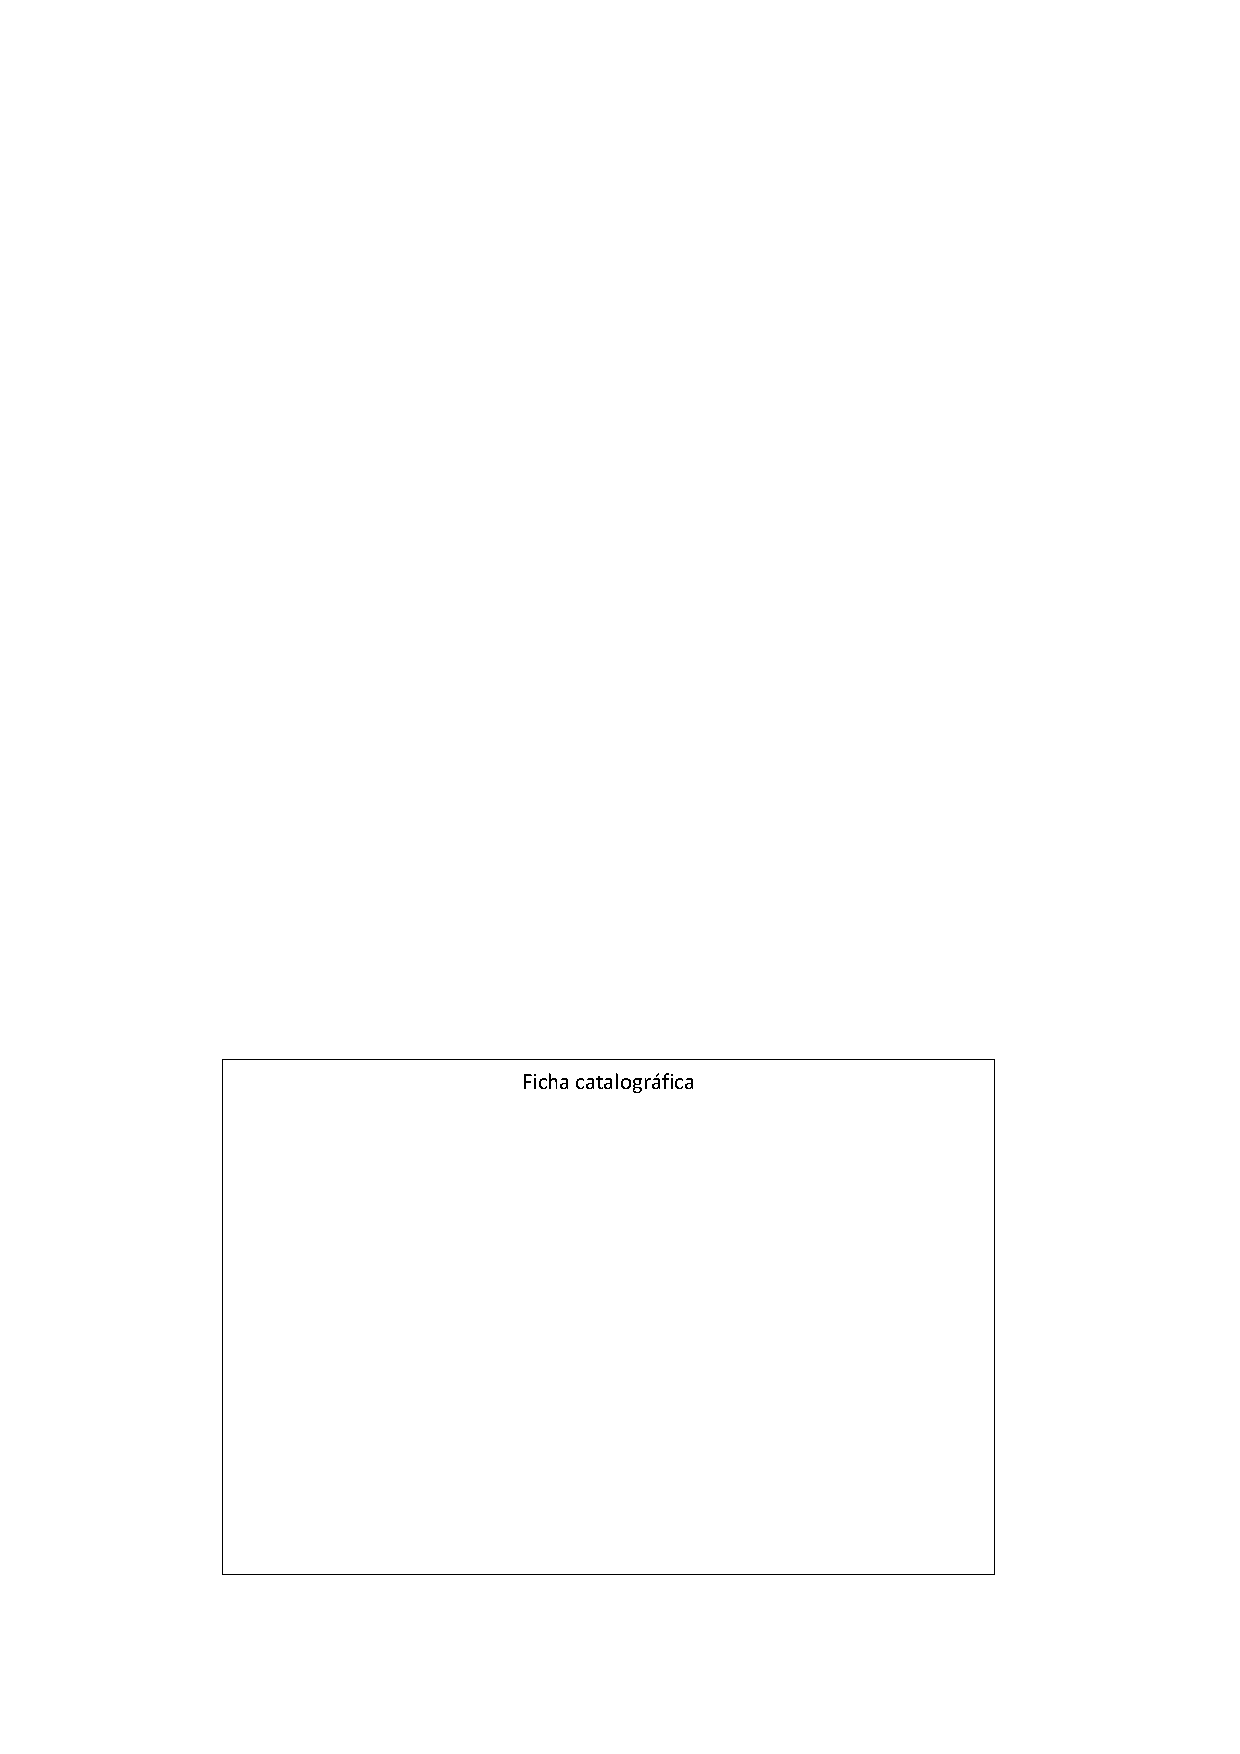
\includepdf{images/fig_ficha_catalografica.pdf}
\end{fichacatalografica}

% ----------------------------------------------------------------------
% Errata (optional)
% ----------------------------------------------------------------------

\begin{errata}
  \noindent
  This is the development version of the thesis (version <1.0.0). Any necessary corrections will be listed here after its approval.
\end{errata}

% ----------------------------------------------------------------------
% Approval sheet (mandatory)
% ----------------------------------------------------------------------

\begin{folhadeaprovacao}
\noindent
[TYPE OF EXAM] exam text by [AUTHOR'S FULL NAME], under the title \textbf{``\imprimirtitulo''}, presented to the [SCHOOL/DEPARTMENT] at the University of São Paulo, as part of the requirements for the degree of [TYPE OF DEGREE] by the [GRADUATE PRGRAM], in the concentration area of [CONCENTRATION AREA].

% [TYPE OF WORK] by [AUTHOR'S FULL NAME], under the title \textbf{``\imprimirtitulo''}, presented to the [SCHOOL/DEPARTMENT] at the University of São Paulo, as part of the requirements for the degree of [TYPE OF DEGREE] by the [GRADUATE PRGRAM]), in the concentration area of [CONCENTRATION AREA].

\vspace*{1.5cm}

\noindent
Approved on \_\_\_\_\_\_\_\_\_\_\_\_\_\_\_\_\_\_\_\_ , \_\_\_\_\_\_\_\_\_\_ .

\vspace*{1.5cm}

\begin{center}
\noindent Examination committee
\end{center}

\vspace*{0.5cm}

\noindent Committee chair:

\vspace*{0.25cm}

\renewcommand{\arraystretch}{2}
\setlength{\arrayrulewidth}{0pt}
\setlength{\tabcolsep}{0pt}
\noindent
\begin{tabular}{m{2cm} P{14cm}}
  Prof. Dr. & \_\_\_\_\_\_\_\_\_\_\_\_\_\_\_\_\_\_\_\_\_\_\_\_\_\_\_\_\_\_\_\_\_\_\_\_\_\_\_\_\_\_\_\_\_\_\_\_\_\_\_\_\_\_\_ \\
  Institution & \_\_\_\_\_\_\_\_\_\_\_\_\_\_\_\_\_\_\_\_\_\_\_\_\_\_\_\_\_\_\_\_\_\_\_\_\_\_\_\_\_\_\_\_\_\_\_\_\_\_\_\_\_\_\_ \\
\end{tabular}

\vspace*{1cm}

\noindent Examiners:

\vspace*{0.25cm}

\noindent
\begin{tabular}{m{2cm} P{14cm}}
  Prof. Dr. & \_\_\_\_\_\_\_\_\_\_\_\_\_\_\_\_\_\_\_\_\_\_\_\_\_\_\_\_\_\_\_\_\_\_\_\_\_\_\_\_\_\_\_\_\_\_\_\_\_\_\_\_\_\_\_ \\
  Institution & \_\_\_\_\_\_\_\_\_\_\_\_\_\_\_\_\_\_\_\_\_\_\_\_\_\_\_\_\_\_\_\_\_\_\_\_\_\_\_\_\_\_\_\_\_\_\_\_\_\_\_\_\_\_\_ \\
  Evaluation & \_\_\_\_\_\_\_\_\_\_\_\_\_\_\_\_\_\_\_\_\_\_\_\_\_\_\_\_\_\_\_\_\_\_\_\_\_\_\_\_\_\_\_\_\_\_\_\_\_\_\_\_\_\_\_ \\
\end{tabular}

\vspace*{0.5cm}

\noindent
\begin{tabular}{m{2cm} P{14cm}}
  Prof. Dr. & \_\_\_\_\_\_\_\_\_\_\_\_\_\_\_\_\_\_\_\_\_\_\_\_\_\_\_\_\_\_\_\_\_\_\_\_\_\_\_\_\_\_\_\_\_\_\_\_\_\_\_\_\_\_\_ \\
  Institution & \_\_\_\_\_\_\_\_\_\_\_\_\_\_\_\_\_\_\_\_\_\_\_\_\_\_\_\_\_\_\_\_\_\_\_\_\_\_\_\_\_\_\_\_\_\_\_\_\_\_\_\_\_\_\_ \\
  Evaluation & \_\_\_\_\_\_\_\_\_\_\_\_\_\_\_\_\_\_\_\_\_\_\_\_\_\_\_\_\_\_\_\_\_\_\_\_\_\_\_\_\_\_\_\_\_\_\_\_\_\_\_\_\_\_\_ \\
\end{tabular}

\vspace*{0.5cm}

\noindent
\begin{tabular}{m{2cm} P{14cm}}
  Prof. Dr. & \_\_\_\_\_\_\_\_\_\_\_\_\_\_\_\_\_\_\_\_\_\_\_\_\_\_\_\_\_\_\_\_\_\_\_\_\_\_\_\_\_\_\_\_\_\_\_\_\_\_\_\_\_\_\_ \\
  Institution & \_\_\_\_\_\_\_\_\_\_\_\_\_\_\_\_\_\_\_\_\_\_\_\_\_\_\_\_\_\_\_\_\_\_\_\_\_\_\_\_\_\_\_\_\_\_\_\_\_\_\_\_\_\_\_ \\
  Evaluation & \_\_\_\_\_\_\_\_\_\_\_\_\_\_\_\_\_\_\_\_\_\_\_\_\_\_\_\_\_\_\_\_\_\_\_\_\_\_\_\_\_\_\_\_\_\_\_\_\_\_\_\_\_\_\_ \\
\end{tabular}
\end{folhadeaprovacao}

% ----------------------------------------------------------------------
% Inscription (optional)
% ----------------------------------------------------------------------

\begin{dedicatoria}
  \vspace*{\fill}
  \centering
  \noindent
  \textit{
  Insert your dedication/inscription here.
  }
	\vspace*{\fill}
\end{dedicatoria}

% ----------------------------------------------------------------------
% Acknowledgments (optional)
% ----------------------------------------------------------------------

\begin{agradecimentos}
  \noindent
  I would like to acknowledge this awesome \href{https://github.com/danielvartan/tesesusp}{Quarto format}! :)
\end{agradecimentos}

% ----------------------------------------------------------------------
% Epigraph (optional)
% ----------------------------------------------------------------------

\begin{epigrafe}
  \vspace*{\fill}
	\begin{flushright}
	  \textit{Awesome quote} \\
		(Awesome quote citation)
	\end{flushright}
\end{epigrafe}

% ----------------------------------------------------------------------
% Abstract in the vernacular language (mandatory)
% ----------------------------------------------------------------------

\setlength{\absparsep}{18pt}
\begin{resumo}

\begin{flushleft}
[SURNAME], [INITIALS]. ([YEAR]). \textit{[TITLE]} [[TYPE OF THESIS]]. [SCHOOL/DEPARTMENT], University of São Paulo, São Paulo. [THESIS'S URL]
\end{flushleft}

Lorem ipsum dolor sit amet, consectetur adipiscing elit. Pellentesque accumsan rutrum lacus, vitae iaculis nisi bibendum in. Nulla et pellentesque nisl. Proin mollis dui sit amet egestas fermentum. Maecenas eu odio odio. Aenean porta ipsum in mauris pharetra dapibus. Nunc dapibus libero nec dui lacinia, id ultricies lectus maximus. Mauris quis mauris in velit pulvinar rutrum. Cras congue ante in orci luctus placerat. Nullam sit amet nisi augue. Maecenas non ligula eros. Etiam nec dolor a mi bibendum auctor.

Keywords: Keyword 1. Keyword 2. Keyword 3.
\end{resumo}

% ----------------------------------------------------------------------
% Abstract in the foreign language (mandatory)
% ----------------------------------------------------------------------

\begin{resumo}[RESUMO]
\begin{otherlanguage*}{brazil}

\begin{flushleft}
[SOBRENOME], [INICIAIS]. ([ANO]). \textit{[TÍTULO]} [[TIPO DE TESE/DISSERTAÇÃO]]. [ESCOLA/DEPARTAMENTO], Universidade de São Paulo, São Paulo. [URL DA DISSERTAÇÃO/TESE]
\end{flushleft}

Lorem ipsum dolor sit amet, consectetur adipiscing elit. Pellentesque accumsan rutrum lacus, vitae iaculis nisi bibendum in. Nulla et pellentesque nisl. Proin mollis dui sit amet egestas fermentum. Maecenas eu odio odio. Aenean porta ipsum in mauris pharetra dapibus. Nunc dapibus libero nec dui lacinia, id ultricies lectus maximus. Mauris quis mauris in velit pulvinar rutrum. Cras congue ante in orci luctus placerat. Nullam sit amet nisi augue. Maecenas non ligula eros. Etiam nec dolor a mi bibendum auctor.

Palavras-chaves: Palavra-chave 1. Palavra-chave 2. Palavra-chave 3.
\end{otherlanguage*}
\end{resumo}

% ----------------------------------------------------------------------
% List of figures (optional)
% ----------------------------------------------------------------------

\renewcommand{\listfigurename}{LIST OF FIGURES}
\pdfbookmark[0]{\listfigurename}{lof}
\listoffigures*
\cleardoublepage

% ----------------------------------------------------------------------
% List of tables (optional)
% ----------------------------------------------------------------------

\renewcommand{\listtablename}{LIST OF TABLES}
\pdfbookmark[0]{\listtablename}{lot}
\listoftables*
\cleardoublepage

% ----------------------------------------------------------------------
% List of abbreviations and acronyms (optional)
% ----------------------------------------------------------------------

\begin{siglas}
  \item[Abbreviation 1] Abbreviation expanded definition
  \item[Abbreviation 2] Abbreviation expanded definition
  \item[Abbreviation 3] Abbreviation expanded definition
\end{siglas}

% ----------------------------------------------------------------------
% List of symbols (optional)
% ----------------------------------------------------------------------

\begin{simbolos}
  \item[$\Gamma$] Gamma
  \item[$\Lambda$] Lambda
  \item[$\zeta$] zeta
\end{simbolos}

% ----------------------------------------------------------------------
% Table of contents (mandatory)
% ----------------------------------------------------------------------

\renewcommand{\contentsname}{TABLE OF CONTENTS}
\pdfbookmark[0]{\contentsname}{toc}
% \tableofcontents*
\cleardoublepage

\ifdefined\Shaded\renewenvironment{Shaded}{\begin{tcolorbox}[sharp corners, breakable, colback={codebgcolor}, borderline west={3pt}{0pt}{shadecolor}, enhanced, boxrule=0pt, frame hidden]}{\end{tcolorbox}}\fi

\renewcommand*\contentsname{Table of contents}
{
\hypersetup{linkcolor=}
\setcounter{tocdepth}{2}
\tableofcontents
}
\bookmarksetup{startatroot}

\hypertarget{introduction}{%
\chapter{INTRODUCTION}\label{introduction}}

\textual

\begin{tcolorbox}[enhanced jigsaw, bottomrule=.15mm, colback=white, left=2mm, bottomtitle=1mm, breakable, toprule=.15mm, leftrule=.75mm, rightrule=.15mm, colframe=quarto-callout-note-color-frame, opacityback=0, colbacktitle=quarto-callout-note-color!10!white, titlerule=0mm, coltitle=black, title=\textcolor{quarto-callout-note-color}{\faInfo}\hspace{0.5em}{Note}, toptitle=1mm, arc=.35mm, opacitybacktitle=0.6]

The text below is for demonstrative purposes only.

\vspace{5pt}

See \url{https://quarto.org/docs/authoring/markdown-basics.html} to
learn about the basics of Markdown's syntax.

\end{tcolorbox}

\vspace{10pt}

``The activity can be represented by a \emph{general schema of
problem-solving by the method of imaginative conjectures and criticism},
or, as I have often called it, by \emph{the method of conjecture and
refutation}. The schema (in its simplest form) is this

\[
\text{P}_{1} \to \text{TT} \to \text{EE} \to \text{P}_{2} 
\]

\vspace{15pt}

Here \(\text{P}_{1}\) is the \emph{problem} from which we start,
\(\text{TT}\) (the `tentative theory') is the imaginative conjectural
solution which we first reach, for example our first \emph{tentative
interpretation}. \(\text{EE}\) (\emph{`error- elimination'}) consists of
a severe critical examination of our conjecture, our tentative
interpretation: it consists, for example, of the critical use of
documentary evidence and, if we have at this early stage more than one
conjecture at our disposal, it will also consist of a critical
discussion and comparative evaluation of the competing conjectures.
\(\text{P}_{2}\) is the problem situation as it emerges from our first
critical attempt to solve our problems. It leads up to our second
attempt (\emph{and so on}). A satisfactory understanding will be reached
if the interpretation, the conjectural theory, finds support in the fact
that it can throw new light on new problems --- on more problems than we
expected; or if it finds support in the fact that it explains many
sub-problems, some of which were not seen to start with. Thus we may say
that we can gauge the progress we have made by comparing
\(\text{P}_{1}\) with some of our later problems (\(\text{P}_{n}\),
say).''

\vspace{15pt}

\noindent \hspace*{\fill} (Popper 1979, 164)

\begin{figure}

\caption{\label{fig-karl-popper}Karl Popper (July 25, 1902 -- September
17, 1994).\\
One of the 20th century's most influential philosophers of science.}

{\centering 

\begin{figure}[H]

{\centering 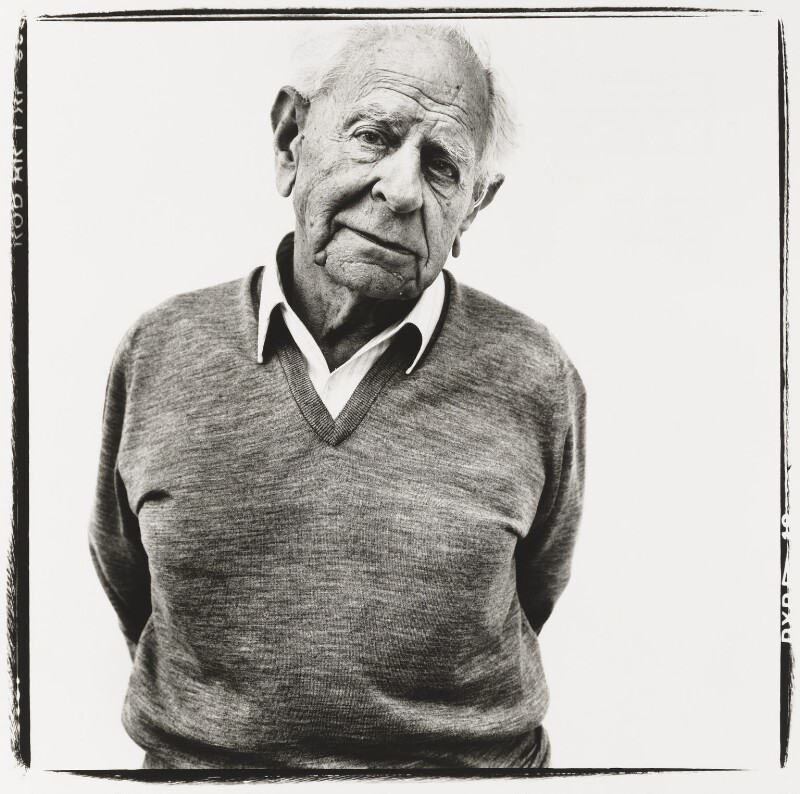
\includegraphics[width=0.5\textwidth,height=\textheight]{images/karl-popper.png}

}

\end{figure}

}

\end{figure}

\hypertarget{secondary-section}{%
\section{SECONDARY SECTION}\label{secondary-section}}

\begin{Shaded}
\begin{Highlighting}[numbers=left,,]
\CommentTok{\# library(datasets)}
\CommentTok{\# library(dplyr)}

\NormalTok{datasets}\SpecialCharTok{::}\NormalTok{iris }\SpecialCharTok{|\textgreater{}}
\NormalTok{  dplyr}\SpecialCharTok{::}\FunctionTok{as\_tibble}\NormalTok{() }\SpecialCharTok{|\textgreater{}}
\NormalTok{  dplyr}\SpecialCharTok{::}\FunctionTok{slice\_sample}\NormalTok{(}\AttributeTok{n =} \DecValTok{5}\NormalTok{)}
\end{Highlighting}
\end{Shaded}

\begin{table}
\caption{A sample of the famous (Fisher's or Anderson's) iris data set}\tabularnewline

\centering
\begin{tabular}{r|r|r|r|l}
\hline
Sepal.Length & Sepal.Width & Petal.Length & Petal.Width & Species\\
\hline
6.5 & 3.0 & 5.5 & 1.8 & virginica\\
\hline
6.5 & 3.0 & 5.8 & 2.2 & virginica\\
\hline
5.0 & 3.0 & 1.6 & 0.2 & setosa\\
\hline
5.0 & 3.5 & 1.6 & 0.6 & setosa\\
\hline
6.2 & 2.9 & 4.3 & 1.3 & versicolor\\
\hline
\end{tabular}
\end{table}

\hypertarget{tertiary-section}{%
\subsection{TERTIARY SECTION}\label{tertiary-section}}

\begin{Shaded}
\begin{Highlighting}[numbers=left,,]
\FunctionTok{plot}\NormalTok{(cars)}
\end{Highlighting}
\end{Shaded}

\begin{figure}[H]

\caption{Speed and stopping distances of cars}

{\centering 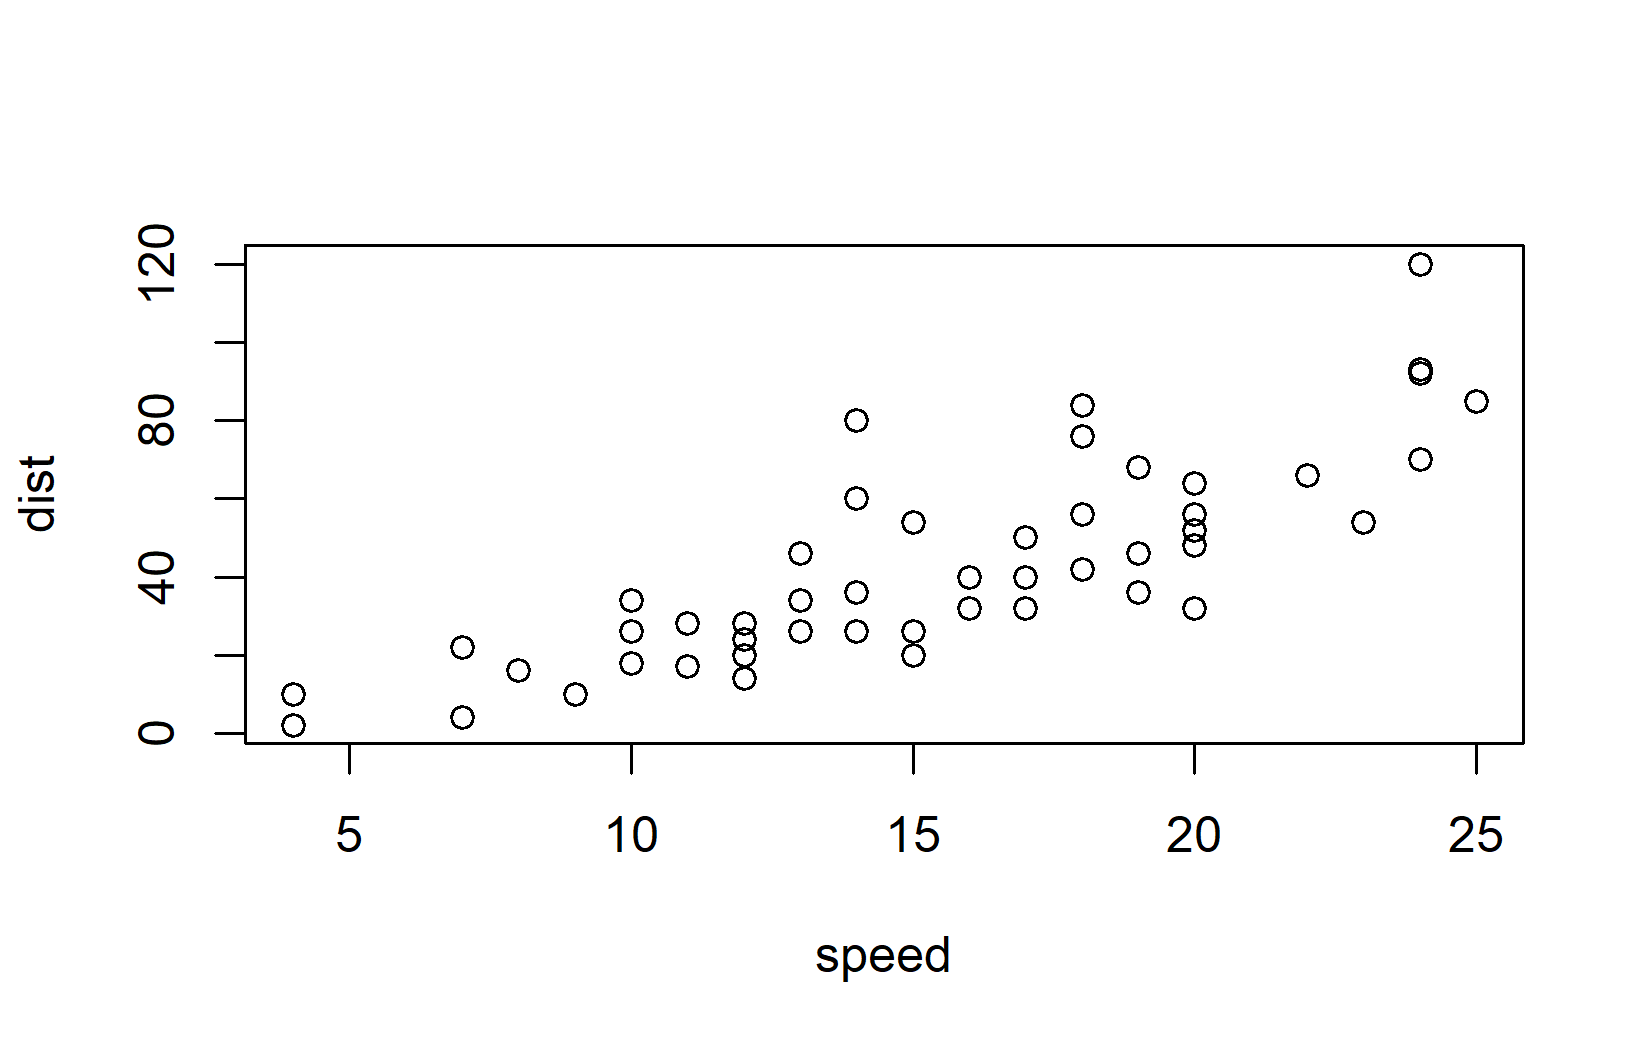
\includegraphics{index_files/figure-pdf/unnamed-chunk-3-1.png}

}

\end{figure}

\hypertarget{quaternary-section}{%
\subsubsection{QUATERNARY SECTION}\label{quaternary-section}}

\begin{itemize}
\tightlist
\item
  Bullet point

  \begin{itemize}
  \tightlist
  \item
    Bullet point

    \begin{itemize}
    \tightlist
    \item
      Bullet point

      \begin{itemize}
      \tightlist
      \item
        Bullet point
      \end{itemize}
    \end{itemize}
  \end{itemize}
\end{itemize}

\bookmarksetup{startatroot}

\hypertarget{development}{%
\chapter{DEVELOPMENT}\label{development}}

\begin{tcolorbox}[enhanced jigsaw, bottomrule=.15mm, colback=white, left=2mm, bottomtitle=1mm, breakable, toprule=.15mm, leftrule=.75mm, rightrule=.15mm, colframe=quarto-callout-warning-color-frame, opacityback=0, colbacktitle=quarto-callout-warning-color!10!white, titlerule=0mm, coltitle=black, title=\textcolor{quarto-callout-warning-color}{\faExclamationTriangle}\hspace{0.5em}{Warning}, toptitle=1mm, arc=.35mm, opacitybacktitle=0.6]

The text below is for demonstrative purposes only.

\vspace{5pt}

See \url{https://quarto.org/docs/authoring/markdown-basics.html} to
learn about the basics of Markdown's syntax.

\end{tcolorbox}

\vspace{10pt}

Lorem ipsum dolor sit amet, consectetur adipiscing elit. Etiam eu mi
massa. Etiam non ipsum ac purus viverra imperdiet a nec quam. Aliquam
tempor ut felis a lacinia. Etiam ut eleifend nisi, non semper est. Nam
lectus lectus, fringilla id blandit a, pellentesque a libero. Curabitur
malesuada mollis porttitor. Mauris lobortis nisi sed semper molestie.
Pellentesque euismod enim nec libero efficitur congue. Nam porta sem sed
dignissim fringilla. Morbi dignissim mi tellus, non egestas velit
vulputate vel. Vivamus ullamcorper rhoncus tellus, in tincidunt leo
fermentum at. Mauris non magna nulla. Donec pulvinar tellus eu nulla
varius placerat. Praesent ut nisi scelerisque, lobortis metus ac, ornare
risus.

Duis erat mi, vulputate eget nibh tempor, pharetra dapibus dolor. Ut
porta, ligula sed mattis interdum, augue felis efficitur dui, vel
imperdiet est ligula ac tellus. Fusce blandit erat id nisl luctus, sit
amet dignissim justo tempor. In rhoncus eleifend velit, sed hendrerit
turpis elementum blandit. In ut rutrum orci. Sed eleifend in tellus
vitae aliquam. Aliquam non velit eleifend diam semper condimentum sit
amet et mi. Morbi ante dui, varius eget leo vel, sodales eleifend
mauris. Curabitur et blandit urna.

\hypertarget{secondary-section-1}{%
\section{SECONDARY SECTION}\label{secondary-section-1}}

Sed placerat elementum sapien et volutpat. Nulla sit amet lacinia leo.
Orci varius natoque penatibus et magnis dis parturient montes, nascetur
ridiculus mus. Donec tempor lacus nec finibus sagittis. Mauris vitae
rutrum nisl. In vestibulum eu risus ac eleifend. In id cursus tellus, ac
vestibulum justo. Praesent convallis a felis semper ultrices. Lorem
ipsum dolor sit amet, consectetur adipiscing elit. In hac habitasse
platea dictumst.

\bookmarksetup{startatroot}

\hypertarget{conclusion}{%
\chapter{CONCLUSION}\label{conclusion}}

\begin{tcolorbox}[enhanced jigsaw, bottomrule=.15mm, colback=white, left=2mm, bottomtitle=1mm, breakable, toprule=.15mm, leftrule=.75mm, rightrule=.15mm, colframe=quarto-callout-important-color-frame, opacityback=0, colbacktitle=quarto-callout-important-color!10!white, titlerule=0mm, coltitle=black, title=\textcolor{quarto-callout-important-color}{\faExclamation}\hspace{0.5em}{Important}, toptitle=1mm, arc=.35mm, opacitybacktitle=0.6]

The text below is for demonstrative purposes only.

\vspace{5pt}

See \url{https://quarto.org/docs/authoring/markdown-basics.html} to
learn about the basics of Markdown's syntax.

\end{tcolorbox}

\vspace{10pt}

Lorem ipsum dolor sit amet, consectetur adipiscing elit. Etiam eu mi
massa. Etiam non ipsum ac purus viverra imperdiet a nec quam. Aliquam
tempor ut felis a lacinia. Etiam ut eleifend nisi, non semper est. Nam
lectus lectus, fringilla id blandit a, pellentesque a libero. Curabitur
malesuada mollis porttitor. Mauris lobortis nisi sed semper molestie.
Pellentesque euismod enim nec libero efficitur congue. Nam porta sem sed
dignissim fringilla. Morbi dignissim mi tellus, non egestas velit
vulputate vel. Vivamus ullamcorper rhoncus tellus, in tincidunt leo
fermentum at. Mauris non magna nulla. Donec pulvinar tellus eu nulla
varius placerat. Praesent ut nisi scelerisque, lobortis metus ac, ornare
risus.

Duis erat mi, vulputate eget nibh tempor, pharetra dapibus dolor. Ut
porta, ligula sed mattis interdum, augue felis efficitur dui, vel
imperdiet est ligula ac tellus. Fusce blandit erat id nisl luctus, sit
amet dignissim justo tempor. In rhoncus eleifend velit, sed hendrerit
turpis elementum blandit. In ut rutrum orci. Sed eleifend in tellus
vitae aliquam. Aliquam non velit eleifend diam semper condimentum sit
amet et mi. Morbi ante dui, varius eget leo vel, sodales eleifend
mauris. Curabitur et blandit urna.

\hypertarget{secondary-section-2}{%
\section{SECONDARY SECTION}\label{secondary-section-2}}

Sed placerat elementum sapien et volutpat. Nulla sit amet lacinia leo.
Orci varius natoque penatibus et magnis dis parturient montes, nascetur
ridiculus mus. Donec tempor lacus nec finibus sagittis. Mauris vitae
rutrum nisl. In vestibulum eu risus ac eleifend. In id cursus tellus, ac
vestibulum justo. Praesent convallis a felis semper ultrices. Lorem
ipsum dolor sit amet, consectetur adipiscing elit. In hac habitasse
platea dictumst.

\bookmarksetup{startatroot}

\hypertarget{references-1}{%
\chapter*{\texorpdfstring{REFERENCES
\footnote{According to the APA style - American Psychological
  Association.}}{REFERENCES }}\label{references-1}}
\addcontentsline{toc}{chapter}{REFERENCES }

\markboth{REFERENCES }{REFERENCES }

\postextual

\hypertarget{refs}{}
\begin{CSLReferences}{1}{0}
\leavevmode\vadjust pre{\hypertarget{ref-popper1979}{}}%
Popper, Karl R. 1979. \emph{Objective Knowledge: An Evolutionary
Approach}. Rev. ed. Oxford University Press.

\end{CSLReferences}

\cleardoublepage
\phantomsection
\addcontentsline{toc}{part}{Appendices}
\appendix

\hypertarget{appendix-1}{%
\chapter{APPENDIX 1}\label{appendix-1}}

\begin{tcolorbox}[enhanced jigsaw, bottomrule=.15mm, colback=white, left=2mm, bottomtitle=1mm, breakable, toprule=.15mm, leftrule=.75mm, rightrule=.15mm, colframe=quarto-callout-tip-color-frame, opacityback=0, colbacktitle=quarto-callout-tip-color!10!white, titlerule=0mm, coltitle=black, title=\textcolor{quarto-callout-tip-color}{\faLightbulb}\hspace{0.5em}{Tip}, toptitle=1mm, arc=.35mm, opacitybacktitle=0.6]

The text below is for demonstrative purposes only.

\vspace{5pt}

See \url{https://quarto.org/docs/authoring/markdown-basics.html} to
learn about the basics of Markdown's syntax.

\end{tcolorbox}

\vspace{10pt}

Lorem ipsum dolor sit amet, consectetur adipiscing elit. Etiam eu mi
massa. Etiam non ipsum ac purus viverra imperdiet a nec quam. Aliquam
tempor ut felis a lacinia. Etiam ut eleifend nisi, non semper est. Nam
lectus lectus, fringilla id blandit a, pellentesque a libero. Curabitur
malesuada mollis porttitor. Mauris lobortis nisi sed semper molestie.
Pellentesque euismod enim nec libero efficitur congue. Nam porta sem sed
dignissim fringilla. Morbi dignissim mi tellus, non egestas velit
vulputate vel. Vivamus ullamcorper rhoncus tellus, in tincidunt leo
fermentum at. Mauris non magna nulla. Donec pulvinar tellus eu nulla
varius placerat. Praesent ut nisi scelerisque, lobortis metus ac, ornare
risus.

Duis erat mi, vulputate eget nibh tempor, pharetra dapibus dolor. Ut
porta, ligula sed mattis interdum, augue felis efficitur dui, vel
imperdiet est ligula ac tellus. Fusce blandit erat id nisl luctus, sit
amet dignissim justo tempor. In rhoncus eleifend velit, sed hendrerit
turpis elementum blandit. In ut rutrum orci. Sed eleifend in tellus
vitae aliquam. Aliquam non velit eleifend diam semper condimentum sit
amet et mi. Morbi ante dui, varius eget leo vel, sodales eleifend
mauris. Curabitur et blandit urna.

\hypertarget{secondary-section-3}{%
\section{SECONDARY SECTION}\label{secondary-section-3}}

Sed placerat elementum sapien et volutpat. Nulla sit amet lacinia leo.
Orci varius natoque penatibus et magnis dis parturient montes, nascetur
ridiculus mus. Donec tempor lacus nec finibus sagittis. Mauris vitae
rutrum nisl. In vestibulum eu risus ac eleifend. In id cursus tellus, ac
vestibulum justo. Praesent convallis a felis semper ultrices. Lorem
ipsum dolor sit amet, consectetur adipiscing elit. In hac habitasse
platea dictumst.



\end{document}
